Testing of AJFS was completed on a small cluster of 8 nodes. Each node in the
cluster was a virtual machine with two cores on a 2.8GHz Intel Xeon CPU. The
systems run Ubuntu 12.04.2 LTS with Linux kernel 3.2.0-39. The nodes each have
2GB of RAM, and share an NFS mounted set of home directories.  Tests were run in
userspace running over NFS. No client-side caching was disabled.

The systems supported FUSE 2.8.6 and Apache Thrift 0.9.0. AJFS was evaluated for
both consistency and performance.

\subsection{Consistency}
The main design goal of AJFS requires file consistency across multiple servers,
and as a result, evaluation of safety and file consistency is the most important
measure of whether AJFS has achieved its objectives.

What follows are the descriptions of a few simple tests and use cases that,
among others, suggest consistency despite a variety of perturbations. 

\subsubsection{Server crash and rejoin}

In distributed system, it's common that a server crashes. We need to guarantee
that when a server is down, data that changes while a server is offline is not
lost, and when the dead server comes back online, the data is synchronized.

% The design of AJFS supports server rejoins. Since it's running based on the
% local backup, client can access the file locally without issue, just like
% Coda~\cite{KS92} does.  The only problem is when the server is down, client
% cannot access the mount point, because fuse server is also down. Instead,
% client should access the local backup. When the server rejoins, it will
% automatiaclly rsync with remote repositories and sync up the local files with
% remote replicas.

Specifically, we tested the following scenario on AJFS:

\begin{enumerate}
    \item AJFS is running with three servers $A$, $B$ and $C$; we kill server
        $C$; client $a$ on server $A$ creates file $x$; we then restart server
        $C$.
    \item AJFS is running with three servers $A$, $B$ and $C$; client $a$
        on server $A$ creates file $x$ and starts writing to it. While writing, we kill server
        $C$. Client $a$ then completes $x$ and we restart server $C$.
\end{enumerate}

In both cases, we were able to successfully retrieve a complete and accurate
file $x$ on server $C$.

The test shows that AJFS is robust against a common occurance: a server dying
while other operations continue. Consistency is still maintained across systems.

\subsubsection{Write protection}

Many distributed systems support mulitple simultaneous writes.
TreadMarks~\cite{treadmarks} supports multiple writers; Bayou~\cite{bayou} askes
each writer to provide dependency check and merge procedures.
However, AJFS choosees to not permit this functionality to avoid the possibility
of conflicts and to maintain simplicity.

A possible solution to support multiple simultaneous writers in AJFS is copy on
write. The write operation only writes to the local copy, and when the file is
closed, the modifications is propagated to the replicas. We do not use this
mechanism because the merge procedure on server the side may be complicated.
Another solution to this issue is to keep different conflict versions of a
single file. 

Instead, we chose locks and only allow one writer to a file at one time, which
is simple and easier to maintain correctness. Given our non-collaborative
expected use cases, this is also completely reasonable.

We tested many cases, drawing special attention to the following cases on AJFS
with two servers $A$ and $B$:
\begin{enumerate}
\item Client $a$ on server $A$ writes to file $x$; at the same time client $b$ on
sever $B$ opens file $x$ for read.
\item Client $a$ on server $A$ writes to file $x$; at the same time client $b$ on
sever $B$ opens file $x$ for write.
\item Client $a$ on server $A$ reads file $x$; at the same time client $b$ on
    sever $B$ deletes the folder which contains file $x$.
\end{enumerate}

On AJFS, all the test cases work as expected; For test case 1, client $b$ can
not open the file for read, because we only allow one writer OR multiple
readers. For test case 2, the request from client $b$ is similarly declined. For
test case 3, AJFS denies the operation, specifying that there are no locks
available. These results suggest that AJFS maintains file consistency in the
presence of multiple interacting clients.

\subsection{Performance}

Performance is \textbf{not} the key motivation of AJFS. Using AJFS to sync up
big files is not efficient as AJFS needs to propagate the data to
all the nodes during the initial write. However, in order to understand how to
improve AJFS, it is useful to understand its current limitations.

Figure~\ref{fig:writeperf} shows the average performance of a \texttt{write()}
under AJFS with a varying number of nodes, as compared with a basic example
using FUSE, and the base file system performance. These values are measured
using the Unix command \texttt{dd}. The results remain consistent regardless of
how much data is written with a single \texttt{write()} call.

There is a clear trend that with the number of AJFS nodes increasing, the write
bandwidth of AJFS decreases. This is because although AJFS uses asynchronous
write propagation in that it does not wait for the response from remote nodes'
operations, it still must transfer the data to other hosts synchronously.
As more nodes means more nodes to transfer to (as each transfer is unicast), the
performance degrades with the number of nodes increasing. 

Figure~\ref{fig:readperf} shows performance of a \texttt{read()} operation under
AJFS with a varying number of nodes. It is constant with respect to the number
of nodes, and is also close to the base FUSE read performance.
This is because AJFS handles \texttt{read()} operations locally and does not
propagate non-modifying requests to other servers.

In both graphs, there is a significant difference in performance between the
local file system and FUSE/AJFS. The version of FUSE used on these systems
clearly adds significant overhead, but this overhead resides in FUSE rather than
in AJFS.

%However, we compare the AJFS system with a local filesystem. The test is run by bonnie++ 1.03e~\cite{bonnie++}. Table \ref{table:performance} shows the AJFS bandwidth performance. 

\begin{figure}[Ht]
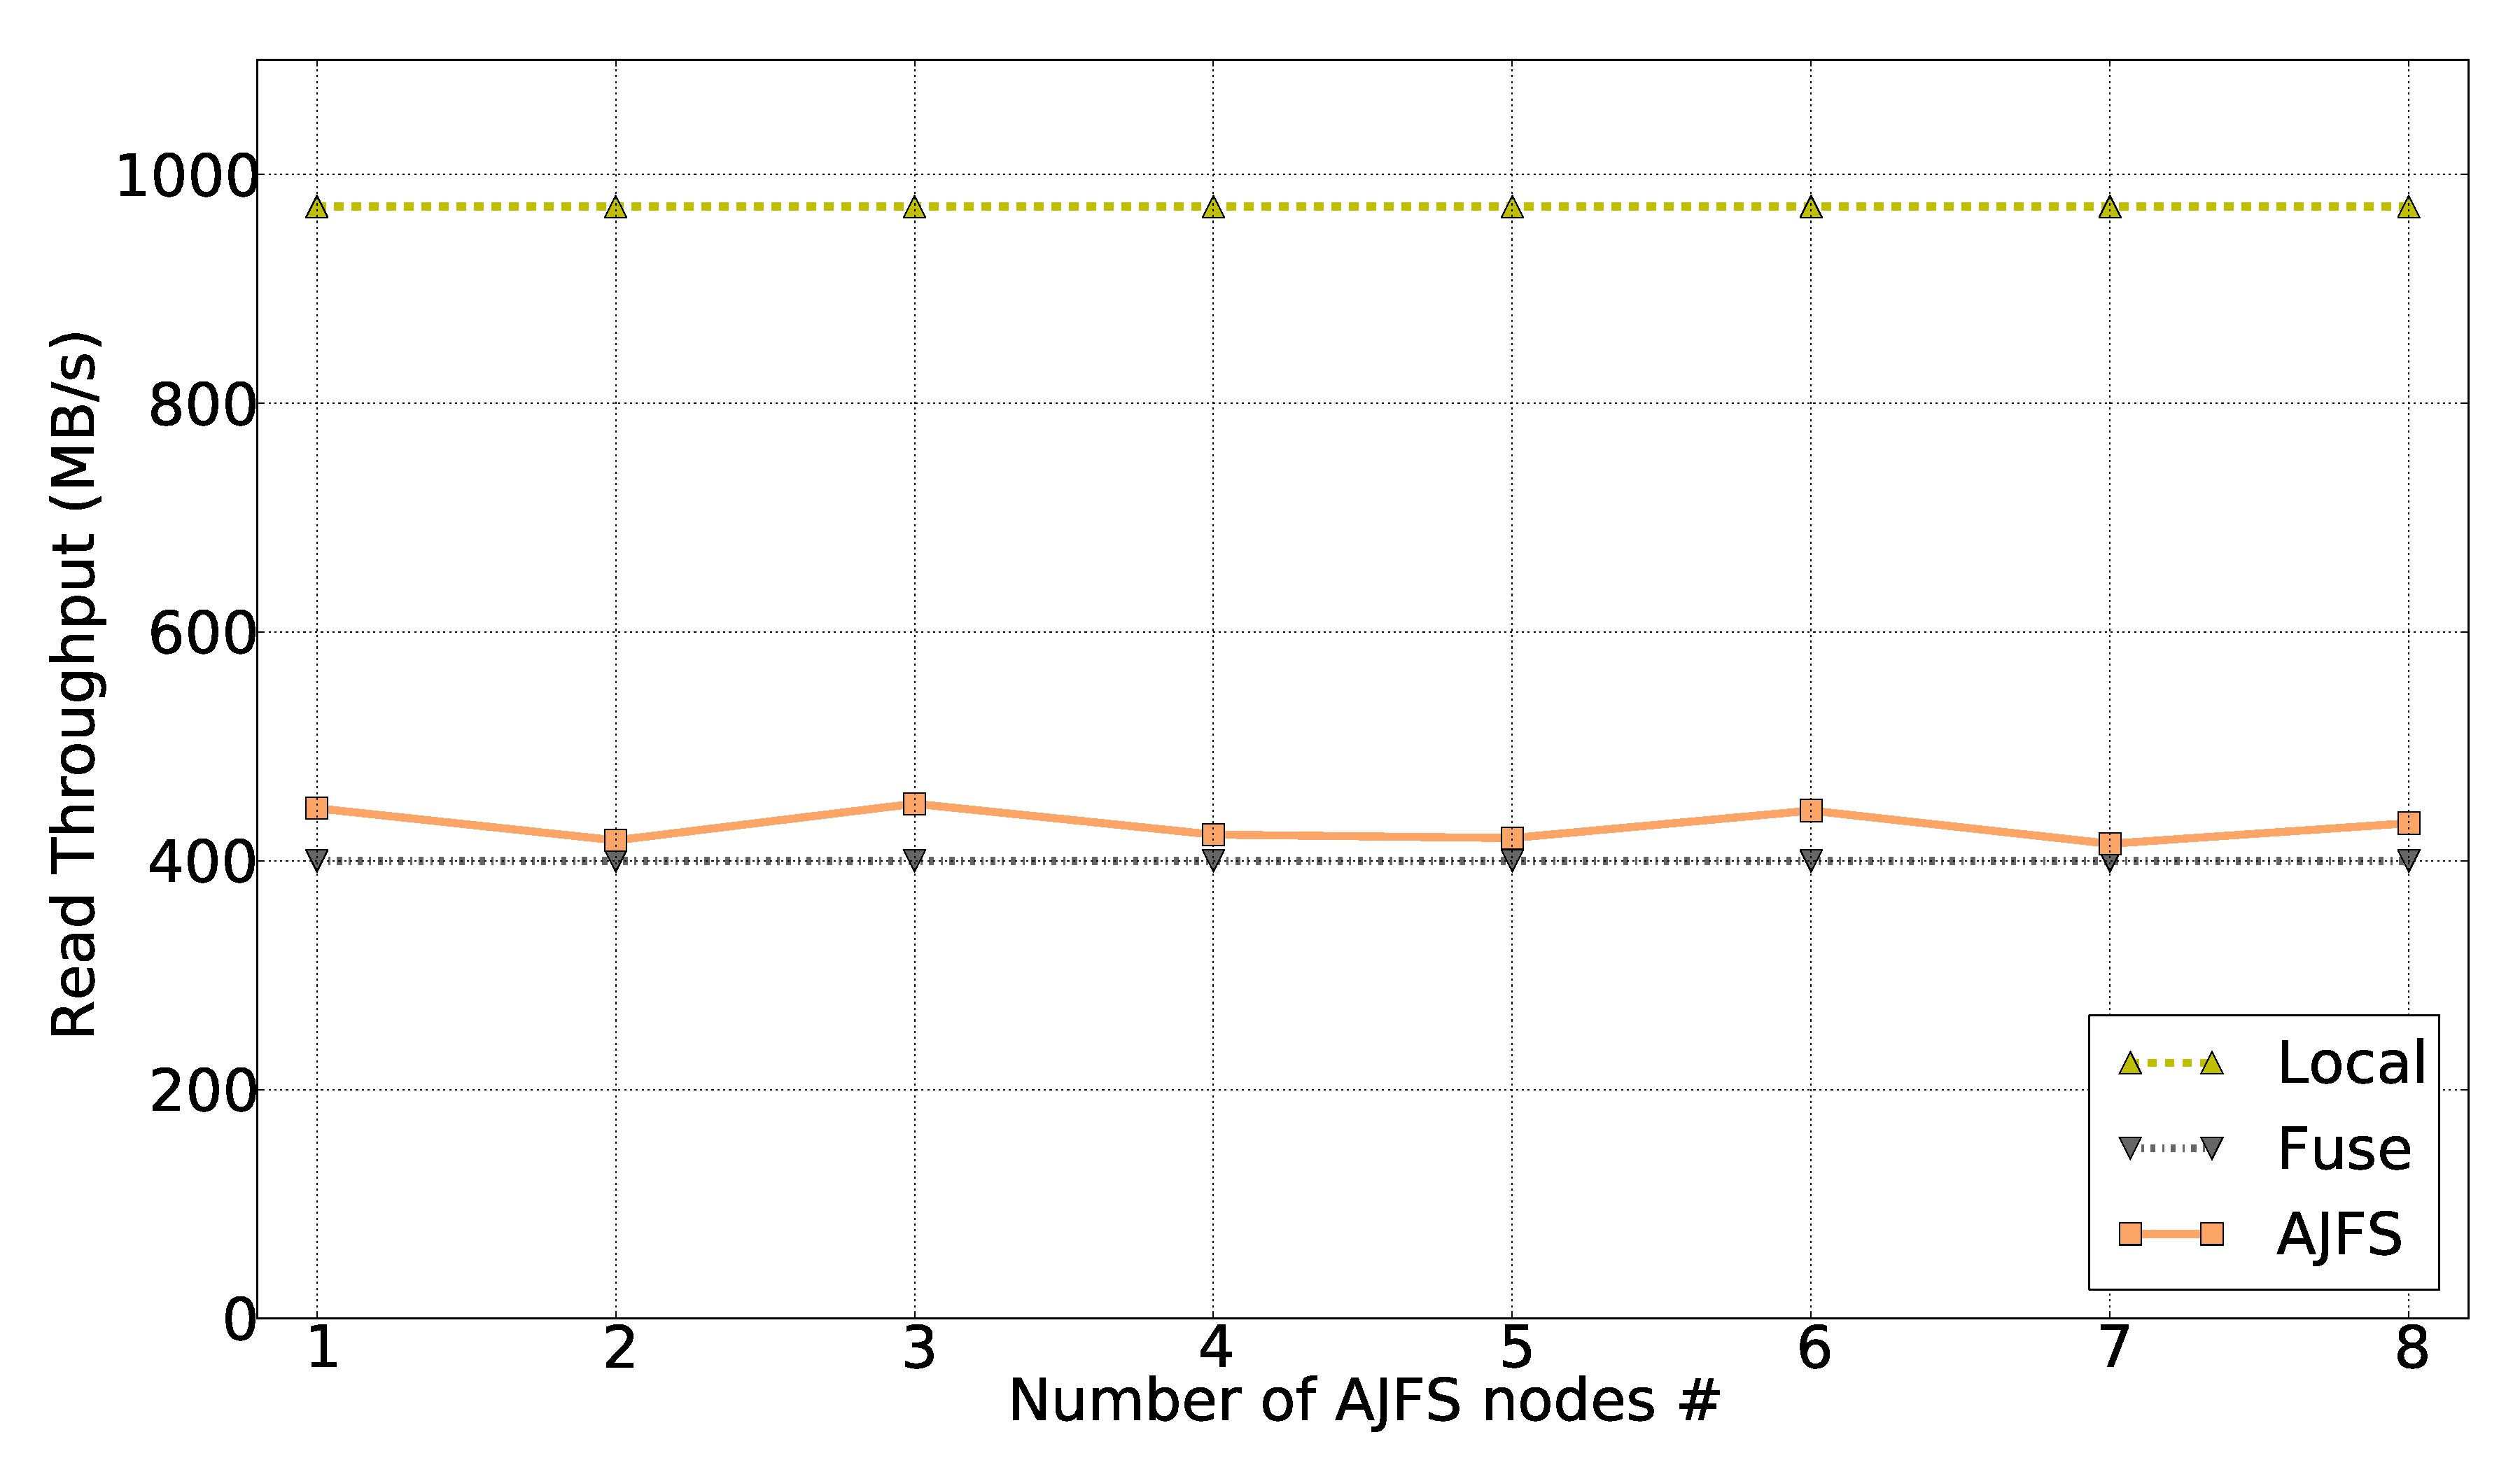
\includegraphics[width=\linewidth]{readperf.pdf}
\caption{AJFS Read Performance}
\label{fig:readperf}
\vspace{-5mm}
\end{figure}

\begin{figure}[Ht]
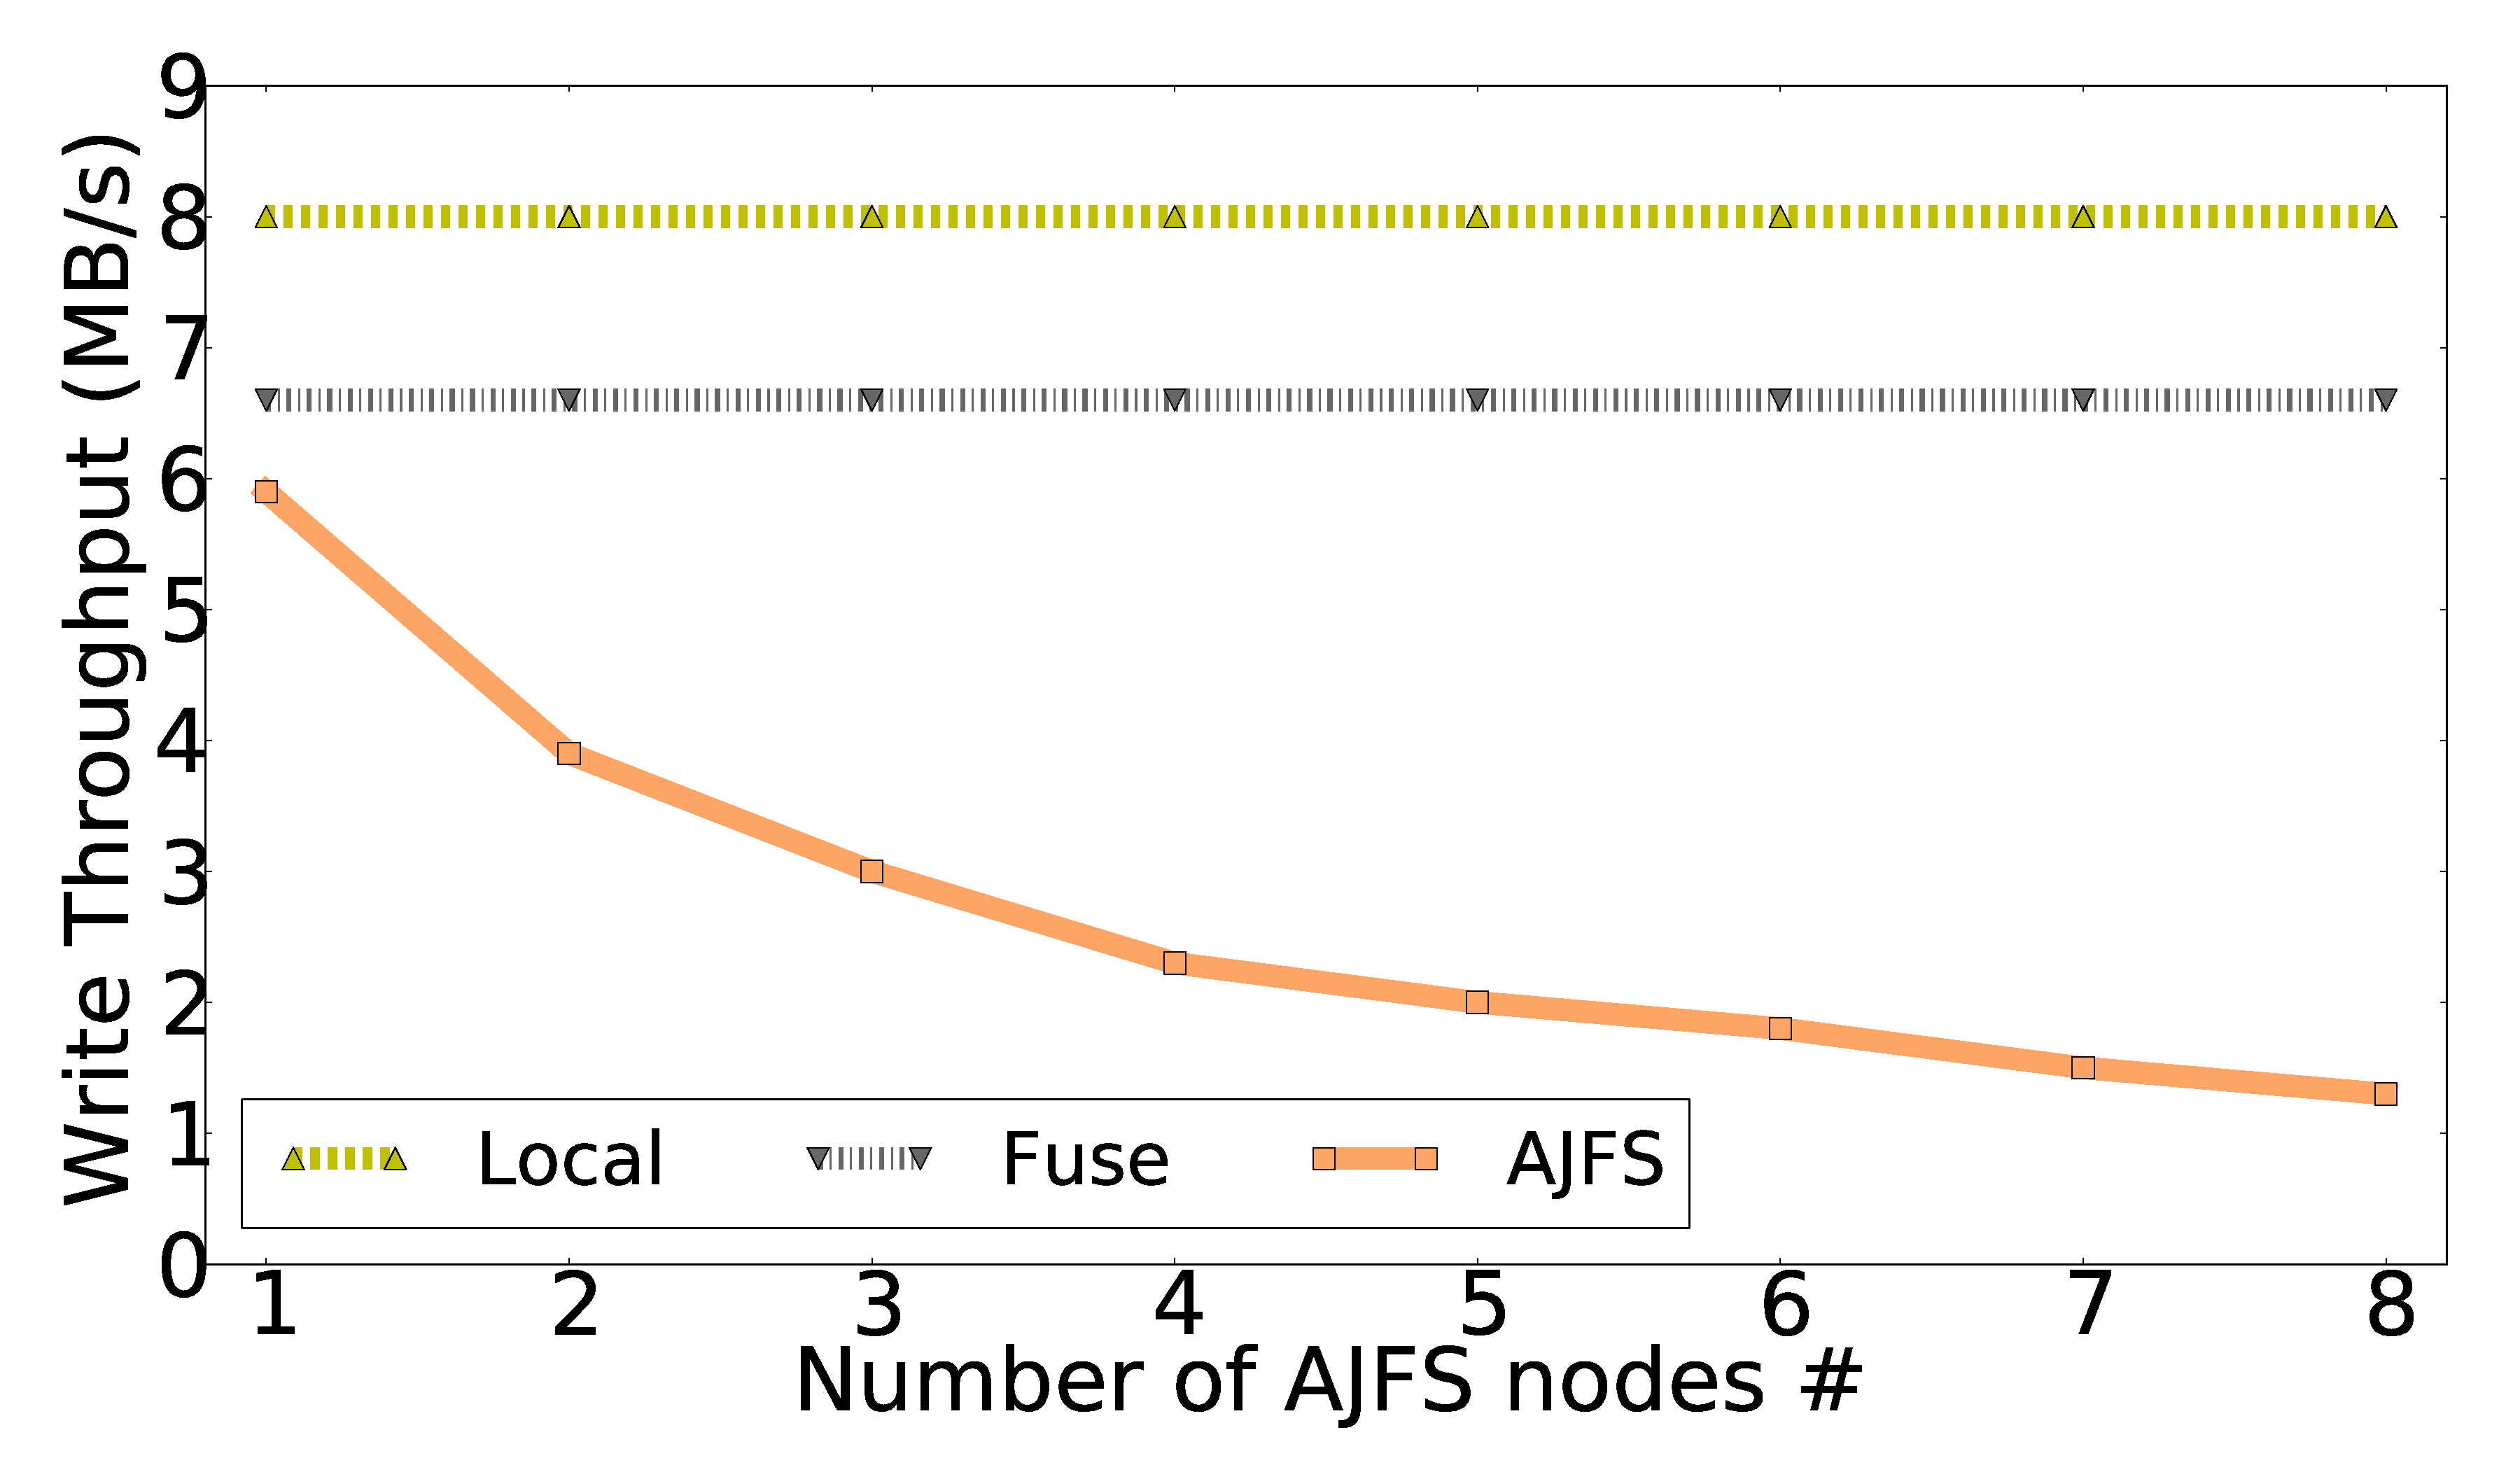
\includegraphics[width=\linewidth]{writeperf.pdf}
\caption{AJFS Write Performance}
\label{fig:writeperf}
\vspace{-5mm}
\end{figure}

%\begin{table}[Ht]
%\caption{AJFS read/write performance (KB/s)}
%\centering
%\begin{tabular}{|p{0.9cm}|p{0.9cm}|p{0.9cm}|p{0.9cm}|p{0.9cm}|p{0.9cm}|}
%\hline\hline
%System & Byte Write & Block Write & Rewrite & Byte Read & Block Read \\
%heading
%\hline
%Ext3	& 49090	& 55403	& 17766	& 45094	& 66464	\\
%\hline
%FUSE	& 33792	& 47490	& 15417	& 39853	& 78666	\\
%\hline
%AJFS	& 13972	& 19651	& 11383	& 41987	& 74125	\\
%\hline
%\end{tabular}
%\label{table:performance}
%\end{table}
